%%%%%%%%%%%%%%%%%%%%%%%%%%%%%%%%%%%%%%%%%
% Beamer Presentation
% LaTeX Template
% Version 1.0 (10/11/12)
%
% This template has been downloaded from:
% http://www.LaTeXTemplates.com
%
% License:
% CC BY-NC-SA 3.0 (http://creativecommons.org/licenses/by-nc-sa/3.0/)
%
%%%%%%%%%%%%%%%%%%%%%%%%%%%%%%%%%%%%%%%%%

%----------------------------------------------------------------------------------------
%	PACKAGES AND THEMES
%----------------------------------------------------------------------------------------

\documentclass{beamer}

\mode<presentation> {

% The Beamer class comes with a number of default slide themes
% which change the colors and layouts of slides. Below this is a list
% of all the themes, uncomment each in turn to see what they look like.

\usetheme{default}
%\usetheme{AnnArbor}
%\usetheme{Antibes}
%\usetheme{Bergen}
%\usetheme{Berkeley}
%\usetheme{Berlin}
%\usetheme{Boadilla}
%\usetheme{CambridgeUS}
%\usetheme{Copenhagen}
%\usetheme{Darmstadt}
%\usetheme{Dresden}
%\usetheme{Frankfurt}
%\usetheme{Goettingen}
%\usetheme{Hannover}
%\usetheme{Ilmenau}
%\usetheme{JuanLesPins}
%\usetheme{Luebeck}
%\usetheme{Madrid}
%\usetheme{Malmoe}
%\usetheme{Marburg}
%\usetheme{Montpellier}
%\usetheme{PaloAlto}
%\usetheme{Pittsburgh}
%\usetheme{Rochester}
%\usetheme{Singapore}
%\usetheme{Szeged}
%\usetheme{Warsaw}

% As well as themes, the Beamer class has a number of color themes
% for any slide theme. Uncomment each of these in turn to see how it
% changes the colors of your current slide theme.

%\usecolortheme{albatross}
%\usecolortheme{beaver}
%\usecolortheme{beetle}
%\usecolortheme{crane}
%\usecolortheme{dolphin}
%\usecolortheme{dove}
%\usecolortheme{fly}
%\usecolortheme{lily}
%\usecolortheme{orchid}
%\usecolortheme{rose}
%\usecolortheme{seagull}
%\usecolortheme{seahorse}
%\usecolortheme{whale}
%\usecolortheme{wolverine}

%\setbeamertemplate{footline} % To remove the footer line in all slides uncomment this line
\setbeamertemplate{footline}[frame number] % To replace the footer line in all slides with a simple slide count uncomment this line


\setbeamertemplate{navigation symbols}{} % To remove the navigation symbols from the bottom of all slides uncomment this line
}
\usepackage[T1]{fontenc}
\usepackage[utf8]{inputenc}
\usepackage{graphicx}
\usepackage{xcolor}
\usepackage{float}
\usepackage{graphicx} % Allows including images
\usepackage{booktabs} % Allows the use of \toprule, \midrule and \bottomrule in tables
\usepackage{tgheros}
\usepackage[defaultmono]{droidmono}

\usepackage{amsmath,amssymb,amsthm,textcomp}
\usepackage{enumerate}
\usepackage{multicol}
\usepackage{tikz}
\usepackage{sidecap}


\usepackage{listings}

\lstset{
language=C++,
basicstyle=\footnotesize\ttfamily,
keywordstyle=\bfseries\color{blue!60!black},
escapechar=@,
commentstyle=\itshape\color{purple!60!black},
showstringspaces=false,
morekeywords={noexcept,constexpr},
breaklines=true}
%basicstyle=\footnotesize\ttfamily}
%tabsize=4,
%aboveskip={1.0\baselineskip},
%belowskip={1.0\baselineskip},
%showtabs=false,
%showspaces=false,
%prebreak=\raisebox{0ex}[0ex][0ex]{\ensuremath{\hookleftarrow}},
%captionpos=t,
%xleftmargin=\parindent}

% code listing settings
%\lstset{
%    language=C++,
%    basicstyle=\ttfamily\small,
%    aboveskip={1.0\baselineskip},
%    belowskip={1.0\baselineskip},
%    columns=fixed,
%    extendedchars=true,
%    breaklines=true,
%    tabsize=4,
%    prebreak=\raisebox{0ex}[0ex][0ex]{\ensuremath{\hookleftarrow}},
%    frame=L,%lines,
%    showtabs=false,
%    showspaces=false,
%    showstringspaces=false,
%    keywordstyle=\bfseries\color{blue!40!black},%\color[rgb]{0.627,0.126,0.941},
%    commentstyle=\itshape\color{purple!40!black},%\color[rgb]{0.133,0.545,0.133},
%    stringstyle=\color{orange},%\color[rgb]{01,0,0},
%    numbers=left,
%    numberstyle=\small,
%    stepnumber=1,
%    numbersep=10pt,
%    captionpos=t,
%    escapeinside={\%*}{*)}
%}

%\lstdefinestyle{customc}{
%  belowcaptionskip=1\baselineskip,
%  breaklines=true,
%  frame=L,
%  xleftmargin=\parindent,
%  language=C,
%  showstringspaces=false,
%  basicstyle=\footnotesize\ttfamily,
%  keywordstyle=\bfseries\color{blue!40!black},
%  commentstyle=\itshape\color{purple!40!black},
%  identifierstyle=\color{blue},
%  stringstyle=\color{orange},
%}




\bibliographystyle{plain}

%----------------------------------------------------------------------------------------
%	TITLE PAGE
%----------------------------------------------------------------------------------------



\author{Florian Frei} % Your name
\date{\today} % Date, can be changed to a custom date

\begin{document}

% Hello and welcome to my midterm presentation
\title{Midterm presentation}
\subtitle{Adaptive Hierarchical Deep Reinforcement Learning}
\begin{frame}
\titlepage
\end{frame}


\begin{frame}[fragile]
\frametitle{Reinforcement Learning}
\includegraphics[scale=0.3]{rl.pdf}
\begin{itemize}
\item Markov Decision Process (MDP) \quad -> 5-tuple $(S, A, P_a, R_a, \gamma)$ \pause
\item Bellmann equation $V^\pi(s)= R(s,\pi(s)) + \gamma \sum_{s'} P(s'|s,\pi(s)) V^\pi(s')$ \pause
\item $\pi^{\ast} = \operatorname{argmax}_{a}{R(s,a) + \gamma \sum_{s'} P(s'|s,a) V^\pi(s')}  $
\end{itemize}
\end{frame}

\begin{frame}[fragile]
\frametitle{Asynchronous Advantage Actor-Critic \footnotemark (A3C) \cite{mnih2016asynchronous}}
\includegraphics[scale=0.3]{a3c.pdf}
\includegraphics[scale=0.6]{actor_critic_arch.pdf}

\footnotetext[1]{Algorithm in Deep Reinforcement Learning (DRL) }
\end{frame}

\begin{frame}
\frametitle{The environment}
A3C was tested on the Arcade Learning Environment (Atari 2600)
\begin{itemize} \pause
\item use gpu for convolution on state images \pause
\item use many cpu cores (16) \pause
\item needs days to converge
\end{itemize}
\end{frame}

\begin{frame}
\frametitle{Toy environment}
\begin{itemize}
\item 1D grid world \pause \qquad -> size variable \pause
\item easy task \pause \qquad -> find the goal \pause
\item fast convergence \pause \qquad -> in hours \pause
\item easy to study \pause \qquad -> handcrafted policies possible \pause
\item only using local cpu's
\end{itemize}
\end{frame}

\begin{frame}[fragile]
\frametitle{Features}
\begin{itemize}
\item local roll-out \pause \qquad -> global update \pause
\item online algorithm  \pause \qquad -> policy \pause
\item learns basic actions from input \pause \qquad  -> no abstraction \pause
\item 2 networks per thread \pause \qquad -> size task specific
\end{itemize}
\end{frame}



\begin{frame}[fragile]
\frametitle{Motivation for more Abstraction}
\begin{itemize}
\item humans learn abstraction automatically \pause
\item dividing the task into subtasks \pause -> learning the subtasks first  \pause
\item humans learn the concept of delayed gratification \pause
\item the further away the goal the higher reward we feel \footnotemark
\end{itemize}
\footnotetext{But learning with sparse rewards is hard}
\end{frame}

\begin{frame}[fragile]
\frametitle{Option-Critic Architecture\footnotemark \cite{bacon2017option}}
\includegraphics[scale=0.8]{option_critic_arch.pdf}
\footnotetext{Algorithm in Hierarchical Deep Reinforcement Learning}
\end{frame}
%-> problem of 1step options
%-> adding delibration cost
%-> epsilon greedy superpolicy


\begin{frame}[fragile]
\frametitle{Problems}
\includegraphics[scale=0.5]{term_problem.pdf}
\begin{itemize}
\item 1-step options \pause \qquad -> instantaneous termination \pause
\item no specialization
\end{itemize}
\end{frame}


\begin{frame}
\frametitle{Option-Critic with delibration cost \cite{harb2017waiting}}
\begin{itemize}
\item current reward $R(s,\pi(s))$ is penalized when the options terminates prematurely before the episode ends \pause
\item to the termination cost a constant term is added for reflecting the cost of switching to another option
\end{itemize}
\end{frame}


\begin{frame}
\frametitle{Open questions}
\begin{itemize}
\item How does the architecture of the options influence the learning process? \pause
\item How does the randomness($\epsilon$) of the super policy influence the learning process? \pause
\item How does the delibration cost influence the learning process? \pause
\item How do the influences above interact with each other?
\end{itemize}
\end{frame}


\begin{frame}
\frametitle{Option architectures}
\begin{itemize}
\item 1 fully connected layer with relu activation and 1 fully connected layer with softmax activation \pause
\item 1 fully connected layer with softmax activation \pause
\item 1 layer without input dependency only 1 bias vector and a softmax activation
\end{itemize}

\end{frame}

\begin{frame}
\frametitle{$\epsilon$-greedy super policy}
\begin{itemize}
\item $\epsilon=0.01$ without annealing \pause
\item $\epsilon=0.1$ without annealing \pause
\item $\epsilon=1.0$ with annealing to $0$ \pause
\item $\epsilon=1.0$ without annealing 
\end{itemize}
\end{frame}

\begin{frame}
\frametitle{Delibration cost}
\begin{itemize}
\item $delib = 0$ \pause
\item $delib = 10^{-1} $ \pause
\item $delib = 10^{-3},10^{-4} $
\end{itemize}

\end{frame}


\begin{frame}
\frametitle{Tensorflow graph}
\includegraphics[scale=0.035]{option_critic_graph_2.png}
\end{frame}


\begin{frame}
\frametitle{Tendencies}
\underline{$\epsilon = 1.0$} \pause
\begin{itemize}
\item equivalent to just pick options randomly \pause
\item all options learn everything if they are able to\pause
\item starting option rarely terminates
\end{itemize}
\end{frame}

\begin{frame}
\frametitle{Tendencies}
Since the task is so simple 1 option with one layer ore more are capable of learning everything.\\ %This implies that the resulting tendencies are also the same.\\
%1 bias option is not capable of learning the optimal policy and needs minimaly 2 options
\underline{$\epsilon = 0.1$}, \underline{$delib = 0$}: \pause
\begin{itemize}
\item $\approx 80$\% is controlled by 1 option rest divided by the others \pause
\item the non dominant options mostly terminate
\end{itemize} \pause
\underline{$\epsilon = 0.1$}, \underline{$delib = 10^{-1}$}: \pause
\begin{itemize}
\item $\approx 99$\% is controlled by 1 option \pause
\item in case the non dominant options are chosen they terminate automatically
\end{itemize} 
\end{frame}

\begin{frame}
\frametitle{Tendencies}

\underline{$\epsilon = 0.1$}, \underline{$delib = 10^{-3},10^{-4}$}: \pause
\begin{itemize}
\item $\approx 68$\% is controlled by 1 option \pause
\item $\approx 19$\% is controlled by another option \pause
\end{itemize}

\underline{$\epsilon = 0.01$}, \underline{$delib = 0 ,10^{-1}, 10^{-3},10^{-4}$}: \pause
\begin{itemize}
\item $\approx 99$\% is controlled by 1 option \pause
\item when not this option is chosen terminate
\end{itemize}

\end{frame}

\begin{frame}
\frametitle{Observations}

$\bullet$ How many options are trained is mainly dependent on two factors. \pause

$\bullet$ When the options are big enough to learn everything for themselves the most important factor is the $\epsilon$ of the super policy which dictates how much knowledge is spread through its randomness.\pause

$\bullet$ When then options are not powerful enough to solve the task completely the super policy learns how many options it needs to solve the task. \pause

$\bullet$ Furthermore since the bias options are decoupled from the input we could observe that the critic(Q value model) was capable of learning the whole task itself. \pause

$\bullet$ But the bias options had to be constructed in such a way that the output vectors were fixed and close to orthogonal. \pause

$\bullet$ In case that they were initialized and trainable the critic we were not yet able to feed the options in such a way, that the options were specialized in a direction of travel.


\end{frame}

\begin{frame}
\bibliography{ref}
\end{frame}

\begin{frame}
\frametitle{QnA}
\end{frame}


\end{document} 